%%%%%%%%%%%%%%%%%%%%%%%%%%%%%%%%%%%%%%%%%%%%%%%%%%%%
% This will help you in writing your homebook
% Remember that the character % is a comment in latex
%
% chapter 3
\chapter{Advanced architecture development}
\label{cha3}

In this section the purpose is to improve the FIR performance. 
\paragraph{}
Initially the unfolding 
technique has been applied to improve the throughput, then pipeline technique has 
been implemented to reduce the critical path and improve the maximum clock frequency.

\section{Unfolding}

Unfolding of order 3 has been applied to FIR filter (N = 3) and the equations derived
to build the new system are the following:

\begin{equation}
\begin{split}
    y[3n] = b_0 \cdot x[3n] + b_1 \cdot x[3(n-1) + 2] + b_2 \cdot x[3(n-1) + 1] + \\
    b_3 \cdot x[3(n-1)] + b_4 \cdot x[3(n-2) + 2] + b_5 \cdot x[3(n-2) + 1] + b_6 \cdot x[3(n-2)] +  \\
    b_7 \cdot x[3(n-3) + 2] + b_8 \cdot x[3(n-3) + 1] + b_9 \cdot x[3(n-3)] + b_{10} \cdot x[3(n-4) + 2]
\end{split}
\end{equation}

\begin{equation}
\begin{split}
    y[3n + 1] = b_0 \cdot x[3n + 1] + b_1 \cdot x[3n] + b_2 \cdot x[3(n-1) + 2] + \\
    b_3 \cdot x[3(n-1) + 1] + b_4 \cdot x[3(n-1)] + b_5 \cdot x[3(n-2) + 2] + b_6 \cdot x[3(n-2)+1] +  \\
    b_7 \cdot x[3(n-2)] + b_8 \cdot x[3(n-3)+2] + b_9 \cdot x[3(n-3) + 1] + b_{10} \cdot x[3(n-3)]
\end{split}
\end{equation}

\begin{equation}
\begin{split}
    y[3n + 2] = b_0 \cdot x[3n + 2] + b_1 \cdot x[3n + 1] + b_2 \cdot x[3n] + b_3 \cdot x[3(n-1) + 2] +\\
    b_4 \cdot x[3(n-1) + 1] + b_5 \cdot x[3(n-1)] + b_6 \cdot x[3(n-2) + 2] +  b_7 \cdot x[3(n-3) + 1] +\\
    b_8 \cdot x[3(n-2)] + b_9 \cdot x[3(n-3) + 2] + b_{10} \cdot x[3(n-3) + 1]
\end{split}
\end{equation}

Using this method of optimization the two more input and output ports have been added because
now 3 inputs are processed and produce, at the same time, 3 outputs. 
\paragraph{}
The overall throughput has
been triplicated with respect to the original architecture.

%% formula dove facciamo vedere che il throuput è triplicato e il nuovo valore calcolato

\section{Pipeline}

A further optimization has been applied. This method allows to reduce the size of the critical path.

From the schematic of the unfolded FIR it is possible to see that to reduce the critical path a chain of registers
is needed to separate the multipliers from the adders. 
\paragraph{}
After these registers are added, the new critical path 
becomes the long chain of adders at the bottom of the scheme.

%image of filter
\centerline{
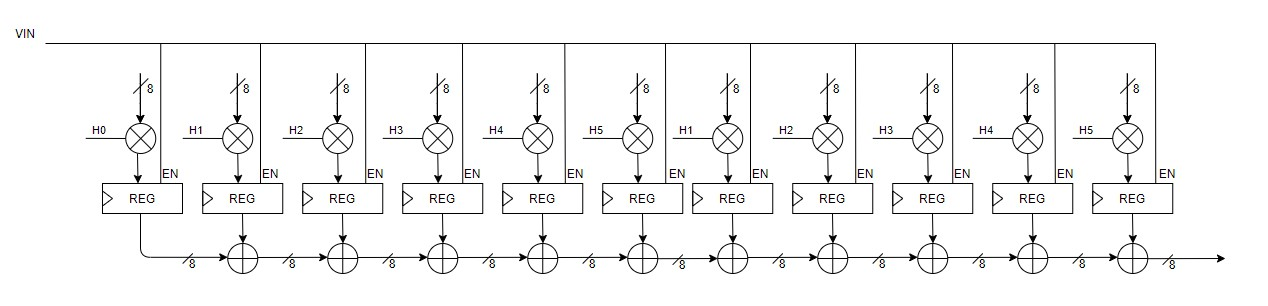
\includegraphics[width=15.5cm]{./chapters/figures/fir_adv_1.jpg}}

\vspace{5mm}

A register is added in the middle of the adder chain; by doing so, it is necessary to delay the stages of the filter
that are positioned behind the new register. Also VIN has to be carefully delayed according to which register it is enabling.
\paragraph{}
After the optimization, the new critical path corresponds to a single multiplier, so it is not possible to improve it more
without adding pipelining to the arithmetic blocks.

\vspace{5mm}
%image of filter
\centerline{
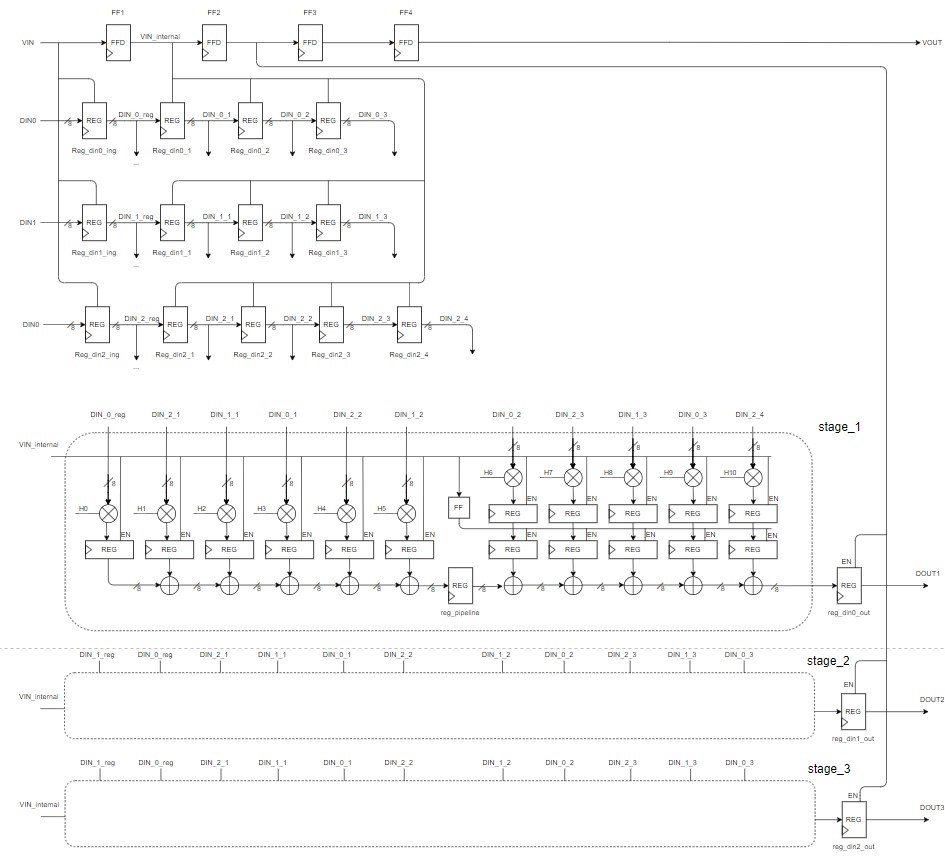
\includegraphics[width=15.5cm]{./chapters/figures/fir_adv_2.jpg}}

\vspace{5mm}

\section{Simulation}

To simulate the advanced implementation of the filter the testbench had to be modified.
\paragraph{} 
The data\_sink and data\_maker were updated in order to be able to transmit and receive 3 inputs every clock cycle.
The first noticiable effect of the optimizations can be noted in the lenght of the Modelsim simulation, which changes from
approximately 2100 ns to 700 ns, a third, as expected due to the increased throughput.

\vspace{5mm}
%image of filter
\centerline{
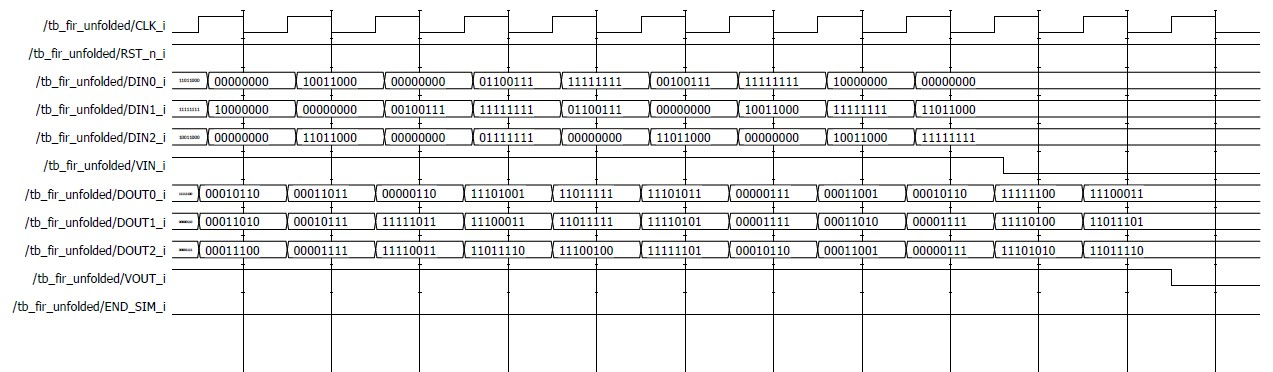
\includegraphics[width=15.5cm]{./chapters/figures/waveform2.jpg}}

\vspace{5mm}

The produced output file has been compared with the results of the C prototype as before, confirming the same behaviour.

\section{Logic synthesis}

The steps performed for the logic synthesis of the base circuit have been repeated to quantify the performance gain.
Running Design Compiler with a timing constraint for the clock period of 0 ns the timing analysis returns the maximum achievable clock frequency,
as well as an area estimation.
\vspace{5mm}

%%table with frequency & area
\centerline{
\begin{tabularx}{1\textwidth} { 
    | >{\centering\arraybackslash}X 
    | >{\centering\arraybackslash}X 
    | >{\centering\arraybackslash}X | }
   \hline
   \textbf{Max Clock Frequency} & \textbf{Min Clock Period} & \textbf{Area} \\
   \hline
   556 MHz  & 1.8 ns  & \unit{14740.4}{\micro\meter\squared}  \\
  \hline
\end{tabularx}}
\vspace{5mm}

This values show that the new architecture is able to work at nearly double the frequency with respect to the previous implementation,
at the expense of a much higher cost in terms of area.

The synthesis is repeated using a clock frequency equal to 25\% of the maximum value previously found.
\vspace{5mm}

\centerline{
\begin{tabularx}{1\textwidth} { 
    | >{\centering\arraybackslash}X 
    | >{\centering\arraybackslash}X 
    | >{\centering\arraybackslash}X | }
   \hline
   \textbf{Clock Frequency} & \textbf{Clock Period} & \textbf{Area} \\
   \hline
   139 MHz  & 7.2 ns  & \unit{13399.5}{\micro\meter\squared}  \\
  \hline
\end{tabularx}}
\vspace{5mm}

The netlist produced by Design Compiler has been used by Modelsim to check the behaviour of the circuit and to annotate the
switching activity of the nodes in a .vcd file. After converting this file to .saif a power estimation was generated by Synopsys.
\vspace{5mm}

\centerline{
\begin{tabularx}{1\textwidth} { 
    | >{\centering\arraybackslash}X 
    | >{\centering\arraybackslash}X 
    | >{\centering\arraybackslash}X
    | >{\centering\arraybackslash}X | }
   \hline
   \multicolumn{4}{|c|}{\textbf{Power [\unit{\micro\watt}]}} \\
   \hline
   \textbf{Internal} & \textbf{Switching} & \textbf{Leakage} & \textbf{Total}\\
   \hline
   1780  & 1170.1  & 277.68 & 3227.8 \\
  \hline
\end{tabularx}}

\vspace{5mm}
The higher number of cells results also in higher power consumption as shown in the previous table. The higher working 
frequency is also a cause for the increase in consumption.

\section{Place \& Route}

The place and route is performed using Innovus on the netlist produced by Synopsys, working at 139 MHz.
The synthesis includes the following steps as shown in the previous chapter:

\begin{itemize}
    \item Structuring the floorplan
    \item Inserting power rings
    \item Standard cell power routing
    \item Placement
    \item Post Clock-Tree-Synthesis optimization
    \item Place filler
    \item Routing
    \item Post routing optimization
    \item Parasitics extraction
    \item Timing analysis
    \item Design analysis and verification
\end{itemize}

\vspace{5mm}
%image of filter
\centerline{
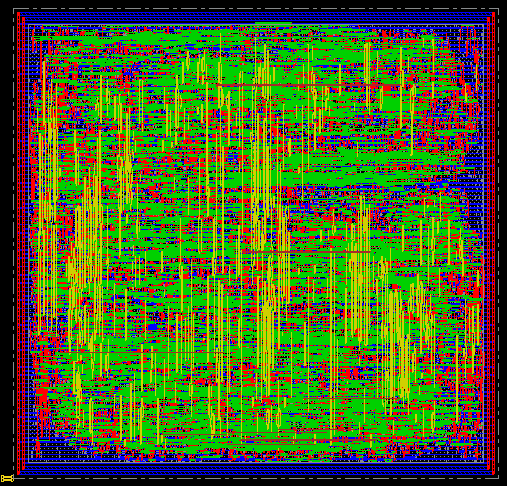
\includegraphics[width=8cm]{./chapters/figures/fir_advanced.png}}

\vspace{5mm}

After verifying that there were no violations in geometry and connections, as well as timing, the netlist with the corresponding
parasitics values was simulated with Modelsim to measure the switching activity of the nodes. The behaviour was checked as well,
confirming the results of the previous simulations.

After restoring the design at the routed level in Innovus, the parasitic values were extracted again and the report power was
produced.

\vspace{5mm}
%tabella con power

\centerline{
\begin{tabularx}{1\textwidth} { 
    | >{\centering\arraybackslash}X 
    | >{\centering\arraybackslash}X 
    | >{\centering\arraybackslash}X 
    | >{\centering\arraybackslash}X | }
    \hline
    \multicolumn{4}{|c|}{\textbf{Power [\unit{\micro\watt}]}} \\
    \hline
    \textbf{Internal} & \textbf{Switching} & \textbf{Leakage} & \textbf{Total}\\
    \hline
    1437  & 796.6  & 258.1 & 2492 \\
   \hline
\end{tabularx}}
\vspace{5mm}

%tabella con area

\centerline{
\begin{tabularx}{0.6\textwidth} { 
    | >{\centering\arraybackslash}X 
    | >{\centering\arraybackslash}X 
    | >{\centering\arraybackslash}X | }
   \hline
   \textbf{Gates} & \textbf{Cells} & \textbf{Area} \\
   \hline
   15844  & 6370  & \unit{12644}{\micro\meter\squared}  \\
  \hline
\end{tabularx}}
\vspace{5mm}

Also in this case Innovus was able to reduce both area and power consumption with respect to the Synopsys evaluation, 
thanks to the various optimization algorithms at its disposal.